\documentclass[aspectratio=169]{beamer} % aspectratio ppt比例

\usetheme{metropolis}           % Use metropolis theme
\usefonttheme[onlymath]{serif}

\usepackage{xeCJK}
\usepackage{graphicx}
\usepackage{amsmath}
\usepackage{multicol}
\usepackage[font=small,labelfont=bf]{caption}
\DeclareCaptionFont{mysize}{\fontsize{7}{9.6}\selectfont}
\captionsetup{font=mysize}

\usepackage{textpos}
\usepackage{adjustbox}
\usepackage{pdfpages}

\newcommand\Fontvi{\fontsize{8}{7.2}\selectfont}

\title{单词相似度计算与短文本对话的研究}
\date{\today}
\author{林连升}
%\institute{福州大学 数学与计算机科学学院}

% title page logo
\titlegraphic{\hspace*{11.2cm} \includegraphics[height=3cm,width=3.38cm]{logo}
}

\begin{document}
  \maketitle

  % frame title logo
  \addtobeamertemplate{frametitle}{}{%
  \begin{textblock*}{100mm}(.96\textwidth,-1.1cm)
  \includegraphics[height=1.2cm,width=1.35cm]{logo}
  \end{textblock*}}

  \begin{frame}{主要工作}
    \begin{itemize}
    \item \textbf{Word Similarity at NLPCC-2016} \newline
    \item \textbf{DBQA at NLPCC-2017} \newline
      Document-Based Question Answering
    \item \textbf{STC-2 at NTCIR-13} \\
      Short Text Conversation
    \end{itemize}
    \end{frame}
  \section{Word Similarity}

    \begin{frame}{数据集: PKU-500}
    \begin{center}
      \begin{figure}
      \includegraphics[width=4in,height=2.2in]{pku-500-1.jpg}
      %\caption{}
      \end{figure}
      \end{center}
    \end{frame}

    \begin{frame}{数据集: PKU-500}
    \begin{center}
      \begin{figure}
      \includegraphics[width=4in,height=2.5in]{pku-500-2.jpg}
      %\caption{}
      \end{figure}
      \end{center}
    \end{frame}

    \begin{frame}{评测指标}
     Spearman's rank correlation coefficient: 
     \begin{equation}
        p = 1 - \frac{6\sum_{i=1}^n{(R_{Xi} - R_{Yi})^2}}{n(n^2 - 1)}
     \end{equation}
     where n is the number of word pairs being evaluated, $R_{Xi}$ and $R_{Yi}$ 
     are the standard deviations of the rank of automatic computing results and 
     human labelled scores, respectively.
    \end{frame}

    \begin{frame}{NLPCC-2016 评测结果}
    \begin{center}
      \begin{figure}
      \includegraphics[width=4in,height=2.8in]{ws-result.png}
      %\caption{}
      \end{figure}
      \end{center}
    \end{frame}

    \begin{frame}{我的结果}
          \begin{table}
      \centering
      %\caption{结果对比}
      \label{tab:commands}
      \begin{minipage}{\columnwidth}
      \begin{center}
      \begin{tabular}{lc}
      \hline
       Method                          &  Spearman \\ \hline
       NLPCC-2016 best result  & 0.518 \\ \hline
       Word2Vec1(2G新闻语料,12对词未覆盖) & 0.338 \\ \hline
       Word2Vec2(2G新闻语料+补充语料)      & 0.400 \\ \hline
       Word2Vec3(20G语料)                & 0.426 \\ \hline
       知网1(刘群等人,2002,118对词未覆盖)    & 0.258  \\ \hline
       知网2(刘群等人,2002,未覆盖给0.5的值)  & 0.418  \\ \hline
       同义词词林(田久乐等人,2010)       & 0.406  \\ \hline
       同义词词林(朱新华等人,2016)       & 0.431  \\ \hline
       Word2Vec2 + 同义词词林2010        & \textbf{0.518}  \\ \hline
       Word2Vec2 + 同义词词林2016        & \textbf{0.538}  \\ \hline
       Word2Vec2 + 同义词词林2010 + 知网1 & \textbf{0.582}  \\ \hline
       Word2Vec2 + 同义词词林2016 + 知网1 & \textbf{0.587}  \\ \hline
      \end{tabular}
      \end{center}
      \end{minipage}
      \end{table}
    \end{frame}

    \begin{frame}{同义词词林}
    参考两篇Paper: 
    \begin{itemize}
      \item [1]田久乐,赵蔚. 基于同义词词林的词语相似度计算方法[J]. 吉林大学学报(信息科学版),2010,06:602-608. \\
      %\item [2]吕立辉,梁维薇,冉蜀阳. 基于词林的词语相似度的度量[J]. 现代计算机(专业版),2013,01:3-6+9. \\
      \item [2]朱新华,马润聪,孙柳,陈宏朝. 基于知网与词林的词语语义相似度计算[J]. 中文信息学报,2016,04:29-36. \\
    \end{itemize}
    \end{frame}

    \begin{frame}{同义词词林简介}
    \begin{center}
      \begin{figure}
      \includegraphics[width=3.1in,height=1.5in]{cilin1.png}
      %\caption{}
      \end{figure}
      \begin{figure}
      \includegraphics[width=4.1in,height=1.2in]{cilin2.png}
      %\caption{}
      \end{figure}
      \end{center}
    \end{frame}

    \begin{frame}{田久乐等的算法,2010}
    \begin{center}
      \begin{itemize}
        \item 主要思想:基于同义词词林的结构, 利用词语中义项的编号, 根据两个义项的语义距离, 计算出义项相似度。\\
        \item 首先判断在同义词林中作为叶子节点的两个义项在哪一层开始分支。例如: Aa01A01与 Aa01B01, 即在第4层分支。在每一层分支,分别对应一个系数,然后再乘以调节参数。\\
      \end{itemize}
    \end{center}
    \end{frame}

    \begin{frame}{田久乐等的算法,2010}
    \begin{center}
      \begin{figure}
      \includegraphics[width=3.9in,height=2in]{cilin-method-2010.png}
      \caption{这里n是分支数,k是两个分支的距离,abcdf是实验得到的系数。}
      \end{figure}
      \end{center}
    \end{frame}

    \begin{frame}{田久乐等的算法,2010}
    举个例子: \\
    Ae05A01= \textcolor{red}{邮递员} \ 邮差 \ 信差 \ 信使 \ 绿衣使者 \ 通信员 \ 投递员 \\
    Ae05A02= 交通员 \ 交通 \ 通讯员 \\
    Ae05A03= \textcolor{red}{联络员} \ 联络官 \ 联系人 \\
    其中,义项“邮递员”和“联络员”在第五层分支,分支数n=3,分支距离k=2,其相似度为:\\
    sim = d * cos(n*pi/180) * ((n-k+1)/n) \\
        = 0.96 * cos(3*pi/180)*((3-2+1)/3) \\
        = 0.639 \\

    \end{frame}

    \begin{frame}{田久乐等的算法, 2010}
    特殊情况: \\
    如果五层编码都相同,则靠末尾的= \# \ @来计算。\\
    \begin{itemize}
      \item =表示同义,相似度取1 \\
      \item \#表示相关,相似度取e(e = 0.5) \\
      \item @表示封闭,只有一个词。因此不存在两个词编号相同且末尾为@的情况。\\
    \end{itemize}

    Ab02A08@ 老太公 \\
    Ab02B01= 成年人 \ 壮年人 \ 大人 \ 人丁 \ 壮丁 \ 佬 \ 中年人 \\
    Ab02C01= 老小 \ 老少 \ 大小 \ 老幼 \ 老老少少 \ 白叟黄童 \ 大大小小 \\
    Ab02C02\# 遗老 \ 遗少 \ 遗老遗少 \ 封建残余 \\
    \end{frame}

    \begin{frame}{朱新华等的算法, 2016}
      \begin{itemize}
        \item (田久乐等,2010)的算法是以分支节点数n和分支间隔k为主要考虑因素,因此会出现许多距离近的词语因分支间隔远而算出相似度过低的不合理现象。为解决这一问题,朱新华等提出了一个以词语距离d为主要影响因素、分支节点数n和分支间隔k为调节参数的计算公式。
        $$
          sim(C_1, C_2) = (1.05 - 0.05dis(C_1, C_2)) \sqrt{e^{\frac{-k}{2n}}}
        $$
      \end{itemize}
    \end{frame}

    \begin{frame}{朱新华等的算法, 2016}
      \begin{itemize}
        \item 其中,$dis(C_1, C_2)$是词语编码$C_1$,$C_2$在树状结构中的距离函数。$W_1$、$W_2$、$W_3$、$W_4$分别为0.5、1、2.5、2.5。因此,距离有1、3、8、13几种情况。
      \end{itemize}
      \begin{figure}
      \includegraphics[width=2.52in,height=1.5in]{cilin2016.png}
      %\caption{}
      \end{figure}
    \end{frame}

    \begin{frame}{《知网》简介}
      \begin{itemize}
        \item 《知网》的结构
          \begin{itemize}
            \item “概念”,是用一种“知识描述语言”来描述的,可以理解为一个词的一种意思。
            \item “义原”,是用于描述一个“概念”的最小语义单位。
          \end{itemize}
      \end{itemize}
      \begin{figure}
      \includegraphics[width=4in,height=1.7in]{hownet1.png}
      %\caption{}
      \end{figure}
      \small
      [3] 刘群, 李素建. 基于《 知网》 的词汇语义相似度计算[J]. 中文计算语言学, 2002.
    \end{frame}

    
    \begin{frame}{知识描述语言的符号及其含义}
      \begin{figure}
      \includegraphics[width=4in,height=1.92in]{hownet3.png}
      %\caption{}
      \end{figure}
    \end{frame}

    \begin{frame}{义原的分类}
      \begin{itemize}
        \item 《知网》一共采用了个1500义原,这些义原分为以下几个大类:
          %\begin{multicols}
          \begin{enumerate}
            \item Event|事件
            \item entity|实体 
            \item attribute|属性
            \item aValue|属性值
            \item quantity|数量
            \item qValue|数量值 
            \item SecondaryFeature|次要特征
            \item syntax|语法
            \item EventRole|事件角色
            \item EventFeatures|事件属性 
          \end{enumerate}
          %\end{multicols}
        \item 这10类义原又分为三组:
          \begin{itemize}
            \item 1-7 基本义原
            \item 8 语法义原
            \item 9、10 关系义原
          \end{itemize}
      \end{itemize}
    \end{frame}

    \begin{frame}{义原的层次结构}
      \begin{columns}
      \begin{column}[t]{0.6\textwidth}
        \begin{itemize}
        \item 在《知网》中,一共描述了义原之间的 8 种关系:上下位关系、同义关系、反义关系、对义关系、 属性-宿主关系、 部件-整体关系、 材料-成品关系、 事件-角色关系。
        \item 根据义原中最重要的上下位关系,所有的“基本义原”组成了一个义原层次体系。
这个义原层次体系是一个树状结构, 也是《知网》进行语义相似度计算的基础。
      \end{itemize}
      \end{column}

      \begin{column}[t]{0.4\textwidth}
        \begin{figure}
      \includegraphics[width=1.6in,height=1.2in]{hownet2.png}
      %\caption{}
      \end{figure}
      \end{column}

      \end{columns}
      
    \end{frame}

    \begin{frame}{知识描述语言归纳}
      \begin{itemize}
        \item 《知网》收录的词语主要分为两类,一类是实词,一类是虚词
        \item 虚词的描述比较简单,用“句法义原”或“关系义原”进行描述
        \item 实词的描述比较复杂,由一系列用逗号隔开的“语义描述式”组成,这些“语义描述式”又有以下三种形式:
          \begin{itemize}
            \item 基本义原描述式:用“基本义原”进行描述;
            \item 关系义原描述式:用“关系义原=基本义原”或者“关系义原=(具体词)”或者“(关系义原=具体词)”来描述;
            \item 关系符号描述式:用“关系符号 \ 基本义原”或者“关系符号(具体词)”加以描述。
          \end{itemize}
      \end{itemize}
    \end{frame}


    \begin{frame}{基于《知网》的词语语义相似度计算方法}
      \begin{itemize}
        \item 词语相似度计算
        \item 义原相似度计算
        \item 虚词概念的相似度计算
        \item 实词概念的相似度计算
      \end{itemize}
    \end{frame}

    \begin{frame}{词语相似度计算}
      对于两个汉语词语$W_1$和$W_2$,如果$W_1$有$n$个概念:$S_1^1$, $S_2^1$,..., $S_n^1$,$W_2$ 有$m$个概念: $S_1^2$, $S_2^2$, ..., $S_m^2$, 规定它们的相似度是各个概念的相似度之最大值:
      \begin{equation}
        Sim(W_1, W_2) = \max_{i=1...n, j=1...m}{Sim(S_i^1, S_j^2)}
      \end{equation}
    \end{frame}

    \begin{frame}{义原相似度计算}
      \begin{itemize}
        \item 由于所有的概念都最终归结于用义原来表示,所以义原的相似度计算是概念相似度计算的基础。
        \item 假设两个义原在树状的层次体系中的路径距离为$d$,我们可以得到这两个义原之间的相似度为:
        \begin{equation}
          Sim(p_1, p_2) = \frac{\alpha}{d + \alpha}
        \end{equation}
      \end{itemize}
    \end{frame}

    \begin{frame}{虚词概念的相似度计算}
      \begin{itemize}
        \item 我们认为,在实际的文本中,虚词和实词总是不能互相替换的,因此,虚词概念和实词概念的相似度总是为零。
        \item 由于虚词概念总是用“语法义原”或“关系义原”这两种方式进行描述,所以,虚词概念的相似度计算归结为,计算其对应的“句法义原”或“关系义原”之间的相似度即可。
      \end{itemize}
    \end{frame}

    \begin{frame}{实词概念的相似度计算}
      实词概念的描述包括两种抽象的结构:集合、特征结构
      \begin{itemize}
        \item 集合 \\
          打:\{exercise|锻炼,sport|体育\}
        \item 特征结构 \\
          写信:\{write|写,ContentProduct=letter|信件\}
      \end{itemize}
    \end{frame}

    \begin{frame}{集合之间的相似度计算}
      \begin{enumerate}
        \item 首先计算两个集合的所有元素两两之间的相似度;
        \item 从所有的相似度值中选择最大的一个记下,将这个相似度值对应的两个元素删除;
        \item 重复上述第 2 步,直到所有的元素都被删除;
        \item 没有建立起对应关系的元素与空元素对应。 
      \end{enumerate}
      集合之间的相似度等于其元素对的相似度的平均值
    \end{frame}

    \begin{frame}{特征结构之间的相似度计算}
      特征结构是“属性-值”对的集合
      \begin{itemize}
        \item 将两个特征结构之间相同的属性一一对应
        \item 计算每个“属性-值”对的相似度,即计算其“值”的相似度
        \item 特征结构之间的相似度就等于所有“属性-值”对的相似度的平均值
      \end{itemize}
    \end{frame}

    \begin{frame}{实词概念的相似度计算}
      实词概念的描述可以表示为一个特征结构,包括以下四个特征:
      \begin{itemize}
        \item 第一基本义原:其值为一个基本义原,这一部分的相似度记为$Sim_1(S_1,S_2)$;
        \item 其它基本义原:除第一基本义原以外的所有基本义原,其值为一个基本义原的集合,这一部分的相似度记为$Sim_2(S_1,S_2)$;
        \item 关系义原描述:对应所有的关系义原描述式,其值是一个特征结构,对于该特征结构的每一个特征,其属性是一个关系义原,其值是一个基本义原,或一个具体词。这一部分的相似度记为$Sim_3(S_1,S_2)$;
        \item 关系符号描述:对应所有的关系符号描述式,其值也是一个特征结构,对于该特征结构的每一个特征,其属性是一个关系义原,其值是一个集合,该集合的每个元素是一个基本义原,或一个具体词。这一部分的相似度记为$Sim_4(S_1,S_2)$。 
    \end{itemize}
    \end{frame}

    \begin{frame}{实词概念的相似度计算}
      \begin{itemize}
        \item 两个概念的总体相似度为:
        \begin{equation}
          Sim(S_1, S_2) = \sum_{i=1}^4 {\beta}_i Sim_i(S_1, S_2)
        \end{equation}
        \item 其中,${\beta}_i (1 \leq i \leq 4)$是可调节的参数,且有:${\beta}_1+{\beta}_2+{\beta}_3+{\beta}_4=1$,${\beta}_1 \geq {\beta}_2 \geq {\beta}_3 \geq {\beta}_4$
        \item 后者反映了$Sim_1$到$Sim_4$ 对于总体相似度所起到的作用依次递减。
    \end{itemize}
    \end{frame}

  \section{Open Domain Question Answering}
  \begin{frame}{ODQA@NLPCC-2017}
    \begin{itemize}
    \item \textbf{NLPCC} \newline
    \textcolor{red}{N}atural \textcolor{red}{L}anguage \textcolor{red}{P}rocessing and \textcolor{red}{C}hinese \textcolor{red}{C}omputing \newline 
    \item \textbf{Open Domain Question Answering} \newline
    including three tasks:
      \begin{itemize}
        \item Knowledge-Based Question Answering (KBQA)
        \item \textbf{Document-Based Qestion Answering (DBQA)}
        \item Table-Based Question Answering (TBQA)
      \end{itemize}
    \end{itemize} 
  \end{frame}

  \begin{frame}{DBQA}
    The task of DBQA is to answer Chinese questions by selecting one or multiple sentences from a given document as answers. \newline
    \begin{center}
      \begin{figure}
      \includegraphics[width=\textwidth,height=\textheight,keepaspectratio]{dbqa-example.png}
      \caption{An example for DBQA}
      \end{figure}
    \end{center}
  \end{frame}

  \begin{frame}{Distance-based Word Overlap}
    \begin{enumerate}
      \item Find question word in question and get its position p \newline
      俄罗斯 {} 贝加尔湖 {} 的 {} 面积 {} 有 {} \textcolor{red}{多大} 
      \item Remove stopwords. Get question word list $W$. \newline
      俄罗斯 {} 贝加尔湖 {} 面积 {} \textcolor{red}{多大} \\
      \quad 0 \qquad \qquad 1 \qquad 2 \quad 3 

      \item Assign score for each word $W$ \newline
        \begin{equation}
          s_i = \begin{cases}2^{-|i-p|} & i \ne p \\ 0 & i = p \end{cases}
        \end{equation}
      \item Scoring sentence $ans$ \newline
        $ score(ans) = \sum_{i}^{l} {\delta}_i $, {}{}{} $ {\delta}_i=\begin{cases}s_i & w_i \in ans  \\ 0 & w_i \notin ans \end{cases} $ \\
        $l$ is the length of W, $w_i$ refers to the word in $W$.
    \end{enumerate}
  \end{frame}

  \begin{frame}{Weighted Distance-based Word Overlap}
    According to whether the word $w_i$ is at the right of the key word or at the left, we update the score computation for the word in $W$ as Eq.4  

      \begin{equation}
      \begin{aligned}
        s_i = \begin{cases} \beta \times 2^{-|i-d|} & i > d \\
         2^{-|i-d|} & i < d \\
         0 & i = d
         \end{cases}
      \end{aligned}
      \end{equation}
    $\beta$ is a positive number tuned by training data. In our experiment, $\beta = 4.3$ is optimized.
  \end{frame}

  \begin{frame}{Experiment}
    \begin{table}
    \centering
    \caption{The result on training data}
    \begin{tabular}{l@{\qquad}l@{\qquad}l}
    \hline\noalign{\smallskip}
    Method & MAP & MRR\\
    \noalign{\smallskip}
    \hline
    \noalign{\smallskip}
    Machine Translation     & 0.2410 & 0.2412  \\
    Average Word Embedding  & 0.4610 & 0.4610  \\
    Paraphrase              & 0.4886 & 0.4906  \\
    Word Overlap            & 0.5114 & 0.5134  \\
    \hline
    Distance-based Overlap  & 0.6848 & 0.6874  \\
    Weighted Distance-based Overlap   & 0.7266 & 0.7293  \\
    \hline
    \end{tabular}
    \end{table}
  \end{frame}

  \begin{frame}{Official Result}
    \begin{center}
      \begin{figure}
      \includegraphics[width=13cm,height=7.45cm]{result-dbqa.png}
      %\caption{Result for DBQA}
      \end{figure}
    \end{center}
  \end{frame}

  \section{Short Text Conversation}

    \begin{frame}{短文本对话}
      
      \begin{figure}
      \includegraphics[width=10cm,height=5.09cm]{stc2-ir-task.png}
      \caption{基于检索的方法}
      \end{figure}

    \end{frame}

    \begin{frame}{Relevance Assessments}
      Judging criteria:
      \begin{enumerate}
        \item Fluent
        \item Coherent: logically and topically relevant 
        \item Self-sufficient
        \item Substantial
      \end{enumerate}
      If (1) or (2) is false: label = "L0" \\
      else if (3) or (4) is false: label = "L1" \\
      else: label = "L2"
    \end{frame}

    \begin{frame}{Labels}
      \begin{center}
        \begin{figure}
        \includegraphics[width=4in,height=2.25in]{stc-labels.png}
        \caption{Example of a post and its five candidate comments with human annotation. }
        \end{figure}
      \end{center}
    \end{frame}

    \begin{frame}{System Architecture}
      \begin{figure}
      \includegraphics[width=14cm,height=4.63cm]{stc-flow-big.png}
      \caption{System Architecture}
      \end{figure}
    \end{frame}

    \begin{frame}{Preprocessing}
      \begin{itemize}
        \item Traditional-Simplified Chinese conversion
        \item Convert Full-width characters into half-width ones
        \item Word segmentation (PKU standard)
        \item Replace number, time, url with token <\_NUM>, <\_TIME>, <\_URL> respectively
        \item Filter meaningless words and special symbols
      \end{itemize}
    \end{frame}

    {
    \setbeamercolor{background canvas}{bg=}
    \includepdf[pages=1]{test.pdf}
    }

    \begin{frame}{Similarity Features}
      \begin{itemize}
        \item TF-IDF
        \item LSA (Latent Semantic Analysis)
        \item LDA (Latent Dirichlet Allocation)
        \item Word2Vec (skip-gram)
        \item \textbf{LSTM-Sen2Vec }
      \end{itemize}
      We combine each post with its corresponding comments to be a document, then train LSA and LDA models on these documents.
    \end{frame}

    \begin{frame}{LSTM}
      \begin{columns}
      \begin{column}[t]{0.6\textwidth}
        \begin{equation}
           f_t = \sigma(W_f \cdot [h_{t-1}, x_t] + b_f)
        \end{equation}
        \begin{equation}
           i_t = \sigma(W_i \cdot [h_{t-1}, x_t] + b_i)
        \end{equation}
        \begin{equation}
           \tilde{C}_t = tanh(W_C \cdot [h_{t-1}, x_t] + b_C) 
        \end{equation}
        \begin{equation}
           C_t = f_t * C_{t-1} + i_t * \tilde{C}_t
        \end{equation}
        \begin{equation}
           o_t = \sigma(W_o \cdot [h_{t-1}, x_t] + b_o)
        \end{equation}
        \begin{equation}
           h_t = o_t * tanh(C_t)
        \end{equation}
      \end{column}

      \begin{column}[t]{0.4\textwidth}
        \begin{figure}
        \includegraphics[width=1.8in,height=1.1in]{lstm2.png}
        \caption{The LSTM Cell.}
        \end{figure}
      \end{column}

      \end{columns}
      \vspace*{2em}

      \tiny
      Mikolov, Toma's. Statistical Language Models Based on Neural Networks. Ph.D. thesis, Brno University of Technology.(2012)

      Zaremba, Wojciech, I. Sutskever, and O. Vinyals. Recurrent Neural Network Regularization. Eprint Arxiv (2014).
      
    \end{frame}

    \begin{frame}{Attention weight}
      \begin{columns}
      \begin{column}[t]{0.5\textwidth}
        \begin{figure}
        \includegraphics[width=6.4cm,height=4.8cm]{forward.png}
        \caption{Unidirectional weight distribution}
        \end{figure}
      \end{column}

      \begin{column}[t]{0.5\textwidth}
        \begin{figure}
        \includegraphics[width=6.4cm,height=4.8cm]{bidirectional.png}
        \caption{bidirectional weight distribution}
        \end{figure}
      \end{column}

      \end{columns}
    \end{frame}

    \begin{frame}{LSTM-Sen2Vec}
      \begin{columns}
      \begin{column}[t]{0.5\textwidth}
        \begin{figure}
        \includegraphics[width=6.7cm,height=3.2cm]{unilstm.png}
        \caption{The Unidirectional LSTM}
        \end{figure}
      \end{column}

      \begin{column}[t]{0.5\textwidth}
        \begin{figure}
        \includegraphics[width=6cm,height=3.2cm]{bilstm1.png}
        \caption{The Traditional Bidirectional LSTM}
        \end{figure}
      \end{column}

      \end{columns}
    \end{frame}

    \begin{frame}{LSTM-Sen2Vec}
      \begin{figure}
        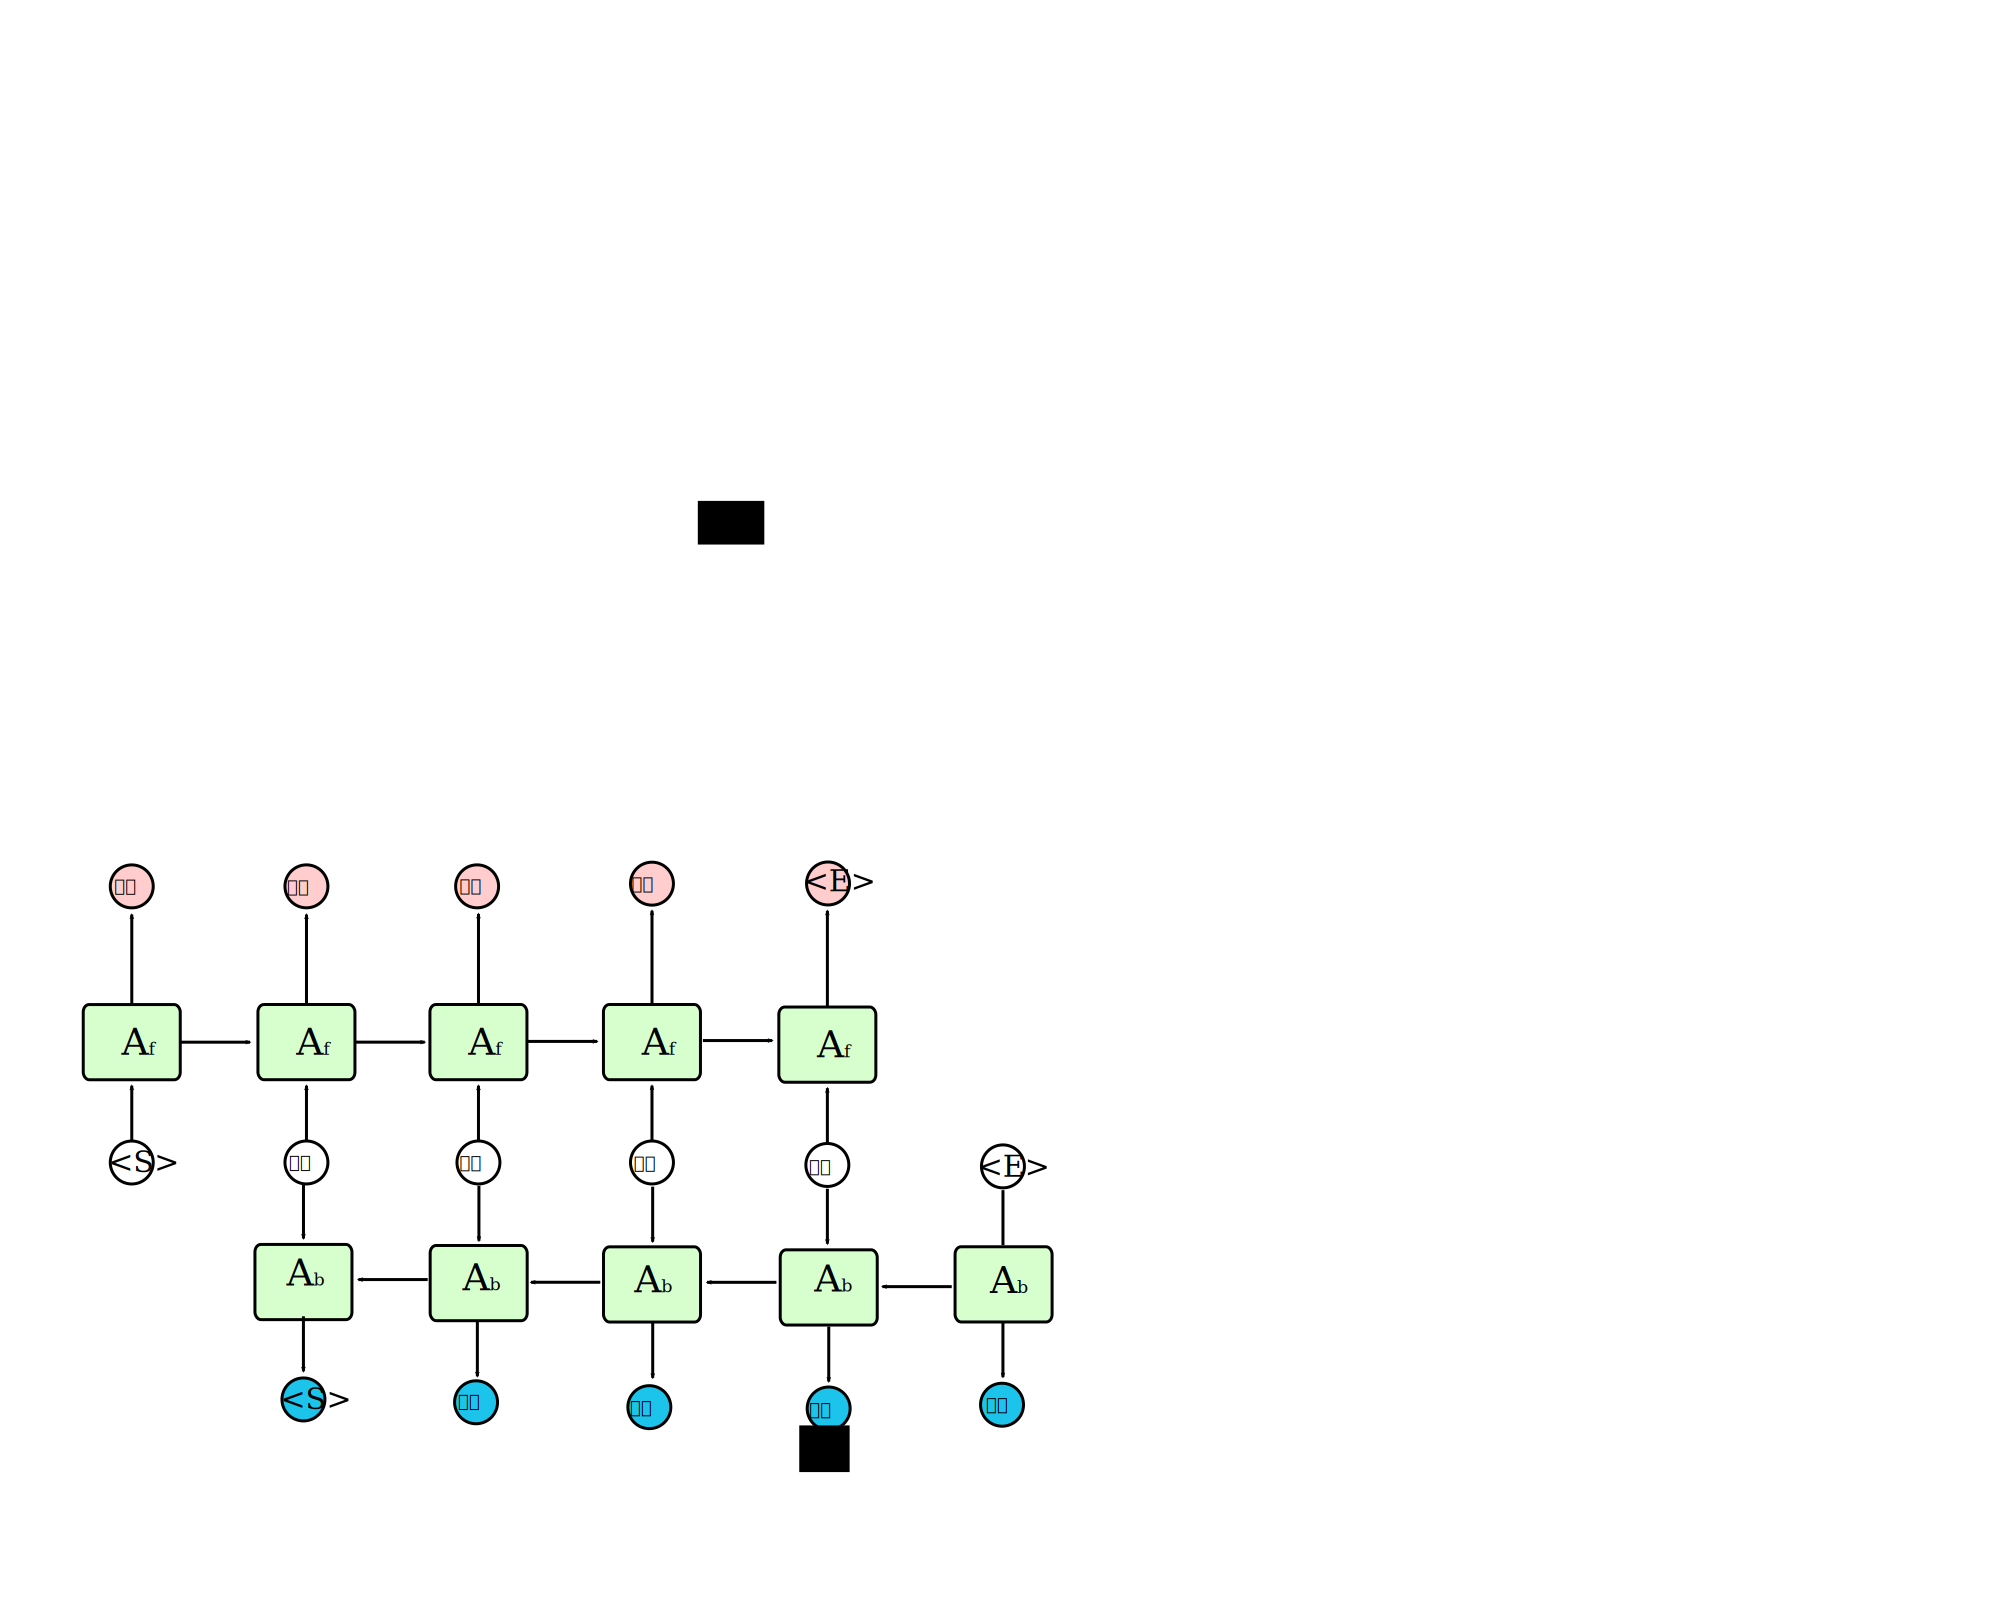
\includegraphics[width=12cm,height=6cm]{bilstm2.png}
        \caption{The Modified Bidirectional LSTM}
        \end{figure}
    \end{frame}

    \begin{frame}{Candidates Generation}
      \begin{itemize}
      \item Similar Posts
      \begin{equation}
         Score_{q,p}^1(q, p) = Sim_{LDA}(q, p) * Sim_{W2V}(q, p) * Sim_{LSTM}(q, p)
      \end{equation}
      \begin{equation}
         Score_{q,p}^2(q, p) = Sim_{LSA}(q, p) * Sim_{W2V}(q, p) * Sim_{LSTM}(q, p)
      \end{equation}
      \item Comment Candidates
      \begin{equation}
         Score_{q,c}^1(q, c) = Sim_{LSA}(q, c) * Sim_{W2V}(q, c)
      \end{equation}
      \begin{equation}
         Score_{q,c}^2(q, c) = Sim_{LDA}(q, c) * Sim_{W2V}(q, c)
      \end{equation}
    \end{itemize}
    \end{frame}

    \begin{frame}{Ranking}
      \begin{itemize}
        \item TextRank (Words as vertices)
        \item Pattern-IDF
        \item Pattern-IDF + TextRank (Sentences as vertices)
      \end{itemize}
    \end{frame}

    \begin{frame}{TextRank - A graph-based ranking model}
      Formally, let $G = (V; E)$ be a undirected graph with the set of vertices 
      $V$ and and set of edges $E$, where $E$ is a subset of $V \times V$. For 
      a given $V_i$, let $link(V_i)$ be the set of vertices that linked with 
      it. The score of a vertex $Vi$ is define as follow:
      \begin{equation}
        WS(V_i) = (1 - d) + d * \sum_{j \in link(V_i)}{w_{ij} * WS{V_j}}
      \end{equation}
      Where $d$ is a damping factor\footnotemark that is usually set to 0.85.

      \footnotetext{Brin, Sergey, and L. Page. The anatomy of a large-scale hypertextual Web search engine. International Conference on World Wide Web Elsevier Science Publishers B. V. 1998:107-117.}
    \end{frame}

    \begin{frame}{TextRank - Vertices and Edges}
      \begin{itemize}
        \item Vertices: each unique word in candidates
        \item Edges: a co-occurrence relation
        \item Weighted by: word2vec similarity between two words and the number of their cooccurrences
      \end{itemize}
    \end{frame}

    \begin{frame}{TextRank - Calculate Iteratively}
      For $N$ candidates, $k$ words in total, we construct $ k \times k $ 
      matrix $M$. $M_{ij} = cnt * sim(D_i, D_j)$. Then we compute iteratively
      \[
      R(t+1) = 
      \begin{bmatrix}
          (1-d)/k       \\
          (1-d)/k       \\
          \hdotsfor{1} \\
          (1-d)/k       
      \end{bmatrix}
      +d
      \begin{bmatrix}
          M_{11} & M_{12} & M_{13} & \dots  & M_{1k} \\
          M_{21} & M_{22} & M_{23} & \dots  & M_{2k} \\
          \vdots & \vdots & \vdots & \ddots & \vdots \\
          M_{k1} & M_{k2} & M_{k3} & \dots  & M_{kk}
      \end{bmatrix}
      R(t)
      \]
      %$R(0) = [IDF(D_0) \ IDF(D_1) \ ... \ IDF(D_{k-1})]^T$ \newline
      Stop when $|R(t+1)-R(t)|<\epsilon$, $\epsilon = 10^{-7}$. \\
      Here, $cnt$ refers to the number of co-ocurrences within a sentence for $D_i$ and $D_j$. \\
    \end{frame}

    \begin{frame}{TextRank - Ranking}
      Since we get the score $R(D_i)$ for each word $D_i$ in candidates, the 
      score for each comment candidate $c$ is calculated as:
      \begin{equation}
        Rank_{TextRank}(c) = \frac{\sum_{D_i \in c}{R(D_i)}}{len(c)} 
      \end{equation}
      where, $len(c)$ refers to the number of words in comment c.
    \end{frame}

    \begin{frame}{Pattern-IDF}
      For word $D_i$ in corresponding comment given word $D_j$ in the post, we define ($D_j$,$D_i$) as a pattern.

      Inspired by the IDF, we calculate the Pattern-IDF as:
      \begin{equation}
        PI(D_i|D_j) = 1 / \log_2{\frac{count_c(D_i) * count_p(D_j)}{count_{pair}(D_i, D_j)}}
      \end{equation}
      where $count_c$ refers to the number of word occurring in comments, $count_p$ refers to that in posts, $count_{pair}$ refers to that in post-comment pair. The PI whose $count_{pair}(D_i, D_j)$ less than 3 are eliminated.

    \end{frame}

    \begin{frame}{Pattern-IDF}
      Let $X = \frac{count_c(D_i) * count_p(D_j)}{count_{pair}(D_i, D_j)}$, then $X \in [1, \infty)$.
      \begin{columns}[T] % align columns
      \begin{column}{.48\textwidth}
      
      \begin{figure}
      \includegraphics[width=6.4cm,height=4.8cm]{pi1.png}
      \caption{log(X)}
      \end{figure}
      
      \end{column}%
      \hfill%
      \begin{column}{.48\textwidth}
      
        \begin{figure}
        \includegraphics[width=6.4cm,height=4.8cm]{pi2.png}
        \caption{1/log(x)}
        \end{figure}

      \end{column}%
      \end{columns}
    \end{frame}

    \begin{frame}{PI - Example}
      \begin{columns}[T] % align columns
      \begin{column}{.48\textwidth}
      \begin{table}[small]
        \centering
        \caption{The example of Pattern-IDF}
        \resizebox{\linewidth}{!}{% Resize table to fit within \linewidth horizontally
        \begin{tabular}{lll}
        \hline
         $Major Word$ & $Minor Word$ & $PI$ \\ \hline
         中国移动 (China Mobile) & 接通 (connect)   & 0.071725 \\ \hline
         中国移动 & cmcc                                  & 0.067261 \\ \hline
         中国移动 & 资费 (charges)   & 0.062408 \\ \hline
         中国移动 & 营业厅 (business hall
        ) & 0.059949 \\ \hline
         中国移动 & 漫游 (roamimg)   & 0.059234 \\ \hline
         ... & ...  & ...  \\ \hline
         中国移动 & 我 (me)   & 0.028889 \\ \hline
         中国移动 & 是 (be)   & 0.027642 \\ \hline
         中国移动 & 的 (of)   & 0.026346 \\ \hline
        \end{tabular}}
        \end{table}
      
      \end{column}%
      \hfill%
      \begin{column}{.48\textwidth}
      \begin{table}[small]
        \centering
        \caption{The entropy of Pattern-IDF for each Major Word}
        \resizebox{.65\linewidth}{!}{% Resize table to fit within \linewidth horizontally
        \begin{tabular}{ll}
        \hline
         $Major Word$   & H \\ \hline
         眼病  (eye disease)     & 0.889971 \\ \hline
         丰收年 (harvest year)      & 0.988191 \\ \hline
         血浆 (plasma)            & 1.033668 \\ \hline
         脊椎动物 (vertebrate)    &  1.083438 \\ \hline
         水粉画 (gouache painting)&  1.180993 \\ \hline
         ...            & ...        \\ \hline
         现在 (now)     & 9.767768   \\ \hline
         什么 (what)  & 10.219045  \\ \hline
         是 (be)         & 10.934950   \\ \hline
        \end{tabular}}
        \end{table}

        
      \end{column}%

      \end{columns}
      
      \begin{equation}
      \Fontvi
      PI_{norm}(D_i|D_j) = \frac{PI(D_i|D_j)}{\sum_{i=1}^n{PI(D_i|D_j)}}
      \end{equation}
      \begin{equation}
      \Fontvi
      H(D_j) = - \sum_{i=1}^n{PI_{norm}(D_i|D_j)\log_2{PI_{norm}(D_i|D_j)}}
      \end{equation}

    \end{frame}

    \begin{frame}{PI - Ranking}
      For each comment $c$ in candidates, given a query (new post) $q$, we 
      calculate the score by $PI$ as follow:
      \begin{equation}
        Score_{PI}(q, c) = \frac{\sum_{D_j \in q}{\sum_{D_i \in c}{PI(D_i|D_j)}}}{len(c) * len(q)}
      \end{equation}
      Then we define rank score as follow:
      \begin{equation}
        Rank_{PI} = (1 + \frac{Score_{PI}(q, c)}{\max{Score_{PI}(q, c)}}) * Sim_{W2V}(q, c)*Sim_{LSA}(q, c)  
      \end{equation}
    \end{frame}

    \begin{frame}{TextRank + Pattern-IDF}
      In this method, We add each comment sentence in candidates as a vertex in the graph and use sentence Word2Vec similarity as edges between vertices in the graph.

      For $N$ candidates, we construct $ N \times N $ matrix $M$. $M_{ij} = SIM_{w2v}(c_i, c_j)$. 

      At time $t = 0$, We initiate a N-dimension vector $P$ , where $N$ is the number 
      of comment candidates. And each entry of $P$ is defined as the score of Pattern-IDF between the query (new post) $q$ and corresponding comment $c_i$ in candidates:
      \begin{equation}
        P_i = Score_{PI}(q, c_i)
      \end{equation}
    \end{frame}

    \begin{frame}{TextRank + Pattern-IDF}
      Then we compute iteratively
      \[
      R(t+1) = 
      \begin{bmatrix}
          (1-d)/N       \\
          (1-d)/N       \\
          \hdotsfor{1} \\
          (1-d)/N       
      \end{bmatrix}
      +d
      \begin{bmatrix}
          M_{11} & M_{12} & M_{13} & \dots  & M_{1N} \\
          M_{21} & M_{22} & M_{23} & \dots  & M_{2N} \\
          \vdots & \vdots & \vdots & \ddots & \vdots \\
          M_{N1} & M_{N2} & M_{N3} & \dots  & M_{NN}
      \end{bmatrix}
      R(t)
      \]
      Stop when $|R(t+1)-R(t)|<\epsilon$, $\epsilon = 10^{-7}$

      Finally, we get the score $P_i$ for each comment in candidates. 
    \end{frame}

  \begin{frame}{Experiment}
    \begin{itemize}
      \item{Nders-C-R5: } LDA + Word2Vec + LSTM-Sen2Vec 
      \item{Nders-C-R4: } LSA + Word2Vec + LSTM-Sen2Vec 
      \item{Nders-C-R3: } R4 + TextRank (Words as vertices)
      \item{Nders-C-R2: } R4 + Pattern-IDF 
      \item{Nders-C-R1: } R4 + Pattern-IDF + TextRank (Sentences as vertices)
    \end{itemize}
  \end{frame}

  \begin{frame}{Official Result}
        \begin{table}
    \centering
    \caption{The official results}
    \label{tab:commands}
    \begin{minipage}{\columnwidth}
    \begin{center}
    \begin{tabular}{|l|c|c|c|}
    \hline
     Run        &  Mean nG@1  &  Mean P+  &  Mean nERR@10  \\ \hline
     SG01 & 0.5867 & 0.6670 & 0.7095 \\ \hline
     splab & 0.5080 & 0.6080 & 0.6492 \\ \hline
     Beihang & 0.4980 & 0.5818 & 0.6105 \\ \hline
     DeepIntell & 0.4323 & 0.5564 & 0.5994 \\ \hline
     Nders-C-R1 & 0.4593 & 0.5394 & 0.5805 \\ \hline
     Nders-C-R2 & 0.4743 & \textbf{0.5497(5th)} & \textbf{0.5882(5th)} \\ \hline
     Nders-C-R3 & 0.4647 & 0.5317 & 0.5768 \\ \hline
     Nders-C-R4 & \textbf{0.4780(4th)} & 0.5338 & 0.5809 \\ \hline
     Nders-C-R5 & 0.4550 & 0.5495 & 0.5868 \\ \hline
     \textcolor{red}{R2 \ vs. \  R4}  & \textcolor{red}{$\downarrow$0.77\%} & \textcolor{red}{$\uparrow$2.98\%} & \textcolor{red}{$\uparrow$1.26\%} \\ \hline

    \end{tabular}
    \end{center}
    \end{minipage}
    \end{table}
  \end{frame}

  \begin{frame}{Example}
    
    \begin{center}
      \begin{figure}
      \includegraphics[width=9.59cm,height=7cm]{stc-result.png}
      \caption{An example for our result}
      \end{figure}
    \end{center}
  \end{frame}

  \begin{frame}[standout]
    Questions?
  \end{frame}

\end{document}

